\section{Application Programming Interfaces}
\label{sec:background:api}

\Glsplx{api} are the interface between a developer needs and the software components at their disposal \citep{Arnold:2005vc} by abstracting the underlying component behind a subroutine, protocol or specific tool. Therefore, it is natural to assess internal quality (and external quality if the software is in itself a service to be used by other developers---in this case an \gls{iws}) is therefore directly related to the quality the \gls{api} offers \citep{Ko:2004td}. 

Good \glspl{api} are known to be intuitive and require less documentation browsing \citep{Piccioni:2013em}, thereby increasing developer productivity. Conversely, poor \glspl{api} are those that are hard to interpret, thereby reducing developer productivity and product quality. The consequences of this have shown a higher demand of technical support (as measured in \citep{Henning:2009hz}) that, ultimately, causes the maintenance to be far more expensive, a phenomenon widely known in software engineering economics (see \cref{ssec:background:software-quality:v-and-v}).

While there are different types of \glspl{api}, such as software library/framework \glspl{api} for building desktop software, operating system \glspl{api} for interacting with the operating system, remote \glspl{api} for communication of varying technologies through common protocols, we focus on web \glspl{api} for communication of resources over the web (being the common architecture of cloud-based services). Being our primary focus, further information on the development, usage and documentation of web \glspl{api} is provided in the below subsection, with a background into \glsac{api} usability in the subsection following.

\subsection{Development, Documentation and Usage of Web APIs}
\label{ssec:background:api:usage}

The development of \textit{web \glsacpl{api}} (commonly referred to as a \textit{web service}) traces its roots back to the early 1990s, where  the Open Software Foundation's \gls{dce} introduced a collection of services and tools for developing and maintaining distributed systems using a client/server architecture \citep{Rosenberry:1992up}. This framework used the synchronous communication paradigm, \glspl{rpc}, that was first introduced by \citet{Nelson:1981ue}. It allows procedures to be called in a remote address space, as if it were local. Its communication paradigm, \gls{dce}/\gls{rpc} \citep{OpenSoftwareFoundation:1991vp}, enables developers to write distributed software with underlying network code abstracted away. To bridge remote \gls{dce}/\glspl{rpc} over components of different operating systems and languages, an \gls{idl} document served as the common service contract or \textit{service interface} for software components. 

This important leap toward language-agnostic distributed programming paved way for \glsac{xml}-\gls{rpc}, enabling \glspl{rpc} over \glsac{http} (and thus the Web) encoded using \glsac{xml} (instead of octet streams \citep{OpenSoftwareFoundation:1991vp}). As new functionality was introduced, this led to the development of the \gls{soap}. This is a backbone messaging connector for web service applications and a realisation of the \gls{soa} \citep{Casati:2003vi} pattern. The \gls{soa} pattern prescribes that services are offered by service providers and consumed by service consumers in a platform- and language-agnostic manner, useful in large-scale enterprise systems (e.g., banking, health). Key to the \gls{soa} pattern is that a service's quality attributes (see \cref{sec:background:software-quality}) can be specified and guaranteed using a \gls{sla} whereby the consumer and provider agree upon a set level of service, which in some cases are legally binding \citep{Bass:2003wi}. This agreement can be measured using \gls{qos} parameters met by the service provider during the transportation layer (e.g., response time, cost of leasing resources, reliability guarantees, system availability and trust/security assurance \citep{Hwang:2017tr,Weerawarana:2005wx}). These attributes are included within \gls{soap} headers; thus, \gls{qos} aspects are independent from the transport layer and instead exist at the application layer \citep{Pautasso2008}. The \gls{idl} of \gls{soap} is \gls{wsdl}, providing a description of how the web service is invoked, what parameters to expect, and what data structures are returned.

\begin{figure}[h!]
  \centering
  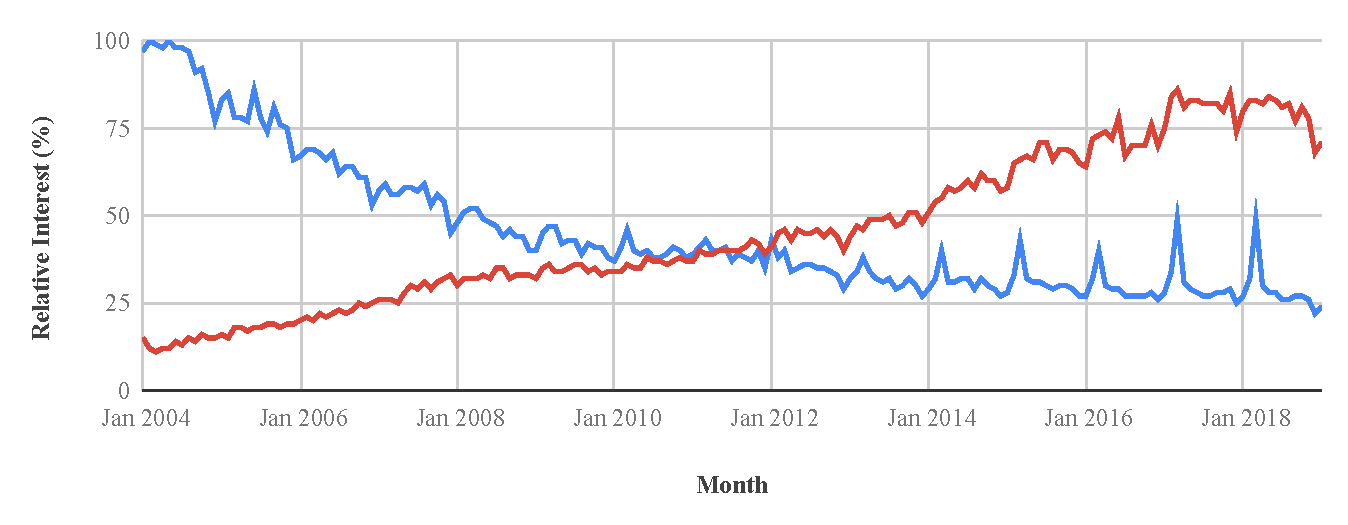
\includegraphics[width=\linewidth]{rest-vs-soap}
  \caption[SOAP versus REST search interest over time]{Worldwide search interest for \glsac{soap} (blue) and \glsac{rest} (red) since 2004. Source: Google Trends.}
  \label{fig:background:apis:rest-vs-soap}
\end{figure}

While it is rich in metadata and verbosity, discussions on whether this was a benefit or drawback came about the mid-2000s \citep{zurMuehlen:2005ci,Pautasso2008}. Namely, it was questioned whether the amount of data transfer happening was worth the verbosity, especially in increasing use of mobile web clients, where data usage over cellular networks was (at the time) scarce and costly. Developer usability for debugging the \gls{soap} `envelopes' (messages \texttt{POST}ed over \glsac{http} to the service provider component) was difficult, both due to the nature of \glsac{xml}'s wordiness and difficulty to test (by sending \texttt{POST} requests) in-browser. As a simple example, 25 lines (794 bytes) of \glsac{http} communication is transferred to request a customer's name from a record using \gls{soap} (\cref{lst:background:apis:soap-request,lst:background:apis:soap-response}). 

\begin{lstlisting}[language=xml,label=lst:background:apis:soap-request,caption={[An example SOAP request]A \gls{soap} \glsac{http} \texttt{POST} consumer request to retrieve customer record \#43456 from a web service provider. Source: \citep{Ballinger:2014aa}.}]
POST /customers HTTP/1.1
Host: www.example.org
Content-Type: application/soap+xml; charset=utf-8

<?xml version="1.0"?>
<soap:Envelope 
  xmlns:soap="http://www.w3.org/2003/05/soap-envelope">
  <soap:Body>
    <m:GetCustomer 
      xmlns:m="http://www.example.org/customers">
      <m:CustomerId>43456</m:CustomerId>
    </m:GetCustomer>
  </soap:Body>
</soap:Envelope>
\end{lstlisting}
\begin{lstlisting}[language=xml,label=lst:background:apis:soap-response,caption={[An example SOAP response]The \gls{soap} \glsac{http} service provider response for \cref{lst:background:apis:soap-request}. Source: \citep{Ballinger:2014aa}.}]
HTTP/1.1 200 OK
Content-Type: application/soap+xml; charset=utf-8

<?xml version='1.0' ?>
<env:Envelope 
  xmlns:env="http://www.w3.org/2003/05/soap-envelope" >
  <env:Body>
    <m:GetCustomerResponse 
      xmlns:m="http://www.example.org/customers">
      <m:Customer>Foobar Quux, inc</m:Customer>
    </m:GetCustomerResponse>
  </env:Body>
</env:Envelope>
\end{lstlisting}

\gls{soap} uses the architectural principle that web services (or the applications they provide) should remain \textit{outside} the web, using \glsac{http} only as a tunnelling protocol to enable remote communication \citep{Pautasso2008}. That is, the \glsac{http} is considered as a transport protocol solely. In 2000, \citet{Fielding:2000vh} introduced \gls{rest}, which instead approaches the web as a medium to publish data (i.e., \glsac{http} is part of the \textit{application} layer instead). Hence, applications become amalgamated into the web. \citeauthor{Fielding:2000vh} bases \gls{rest} on four key principles:

\begin{itemize}
  \item \textbf{\glsacpl{uri} identify resources.} Resources and services have a consistent global address space that aides in their discovery via \glsacpl{uri} \citep{BernersLee:2004vf}.
  \item \textbf{\glsac{http} verbs manipulate those resources.} Resources are manipulated using the four consistent \glsac{crud} verbs provided by \glsac{http}, such as \texttt{POST}, \texttt{GET}, \texttt{PUT}, and \texttt{DELETE}.
  \item \textbf{Self-descriptive messages.} Each request provides enough description and context for the server to process that message.
  \item \textbf{Resources are stateless.} Every interaction with a resource is stateless.
\end{itemize}

\noindent
Consider the equivalent example of \cref{lst:background:apis:soap-request,lst:background:apis:soap-response} but in a \glsac{rest}ful architecture (\cref{lst:background:apis:rest-request,lst:background:apis:rest-response}) and it is clear why this style has grown more popular with developers (as we highlight in \cref{fig:background:apis:rest-vs-soap}). Developers have since embraced \gls{rest}ful \gls{api} development, though the major drawback of \gls{rest}ful services is its lack of a uniform \gls{idl} to facilitate development (though it is possible to achieve this using \gls{wadl} \citep{Mandel:2008ww}).  Therefore, no RESTful service uses a standardised response document or invocation syntax. While there are proposals, such as \gls{wadl} \citep{Hadley:2006vv}, \glsac{raml},\footnoteurl{https://raml.org}{25 January 2019} \gls{api} Blueprint,\footnoteurl{https://apiblueprint.org}{25 January 2019} and the OpenAPI\footnoteurl{https://www.openapis.org}{25 January 2019} specification (initially based on Swagger\footnoteurl{https://swagger.io}{25 January 2019}), there is still no consensus as there was for \gls{soap} and convergence of these \glspl{idl} is still underway.

\begin{lstlisting}[label=lst:background:apis:rest-request,caption={[An example RESTful request]An equivalent \glsac{http} consumer request to that of \cref{lst:background:apis:soap-request}, but using \gls{rest}. Source: \citep{Ballinger:2014aa}.}]
GET /customers/43456 HTTP/1.1
Host: www.example.org
\end{lstlisting}
\begin{lstlisting}[language=json,label=lst:background:apis:rest-response,caption={[An example RESTful response]The \gls{rest} \glsac{http} service provider response for \cref{lst:background:apis:rest-request}.}]
HTTP/1.1 200 OK
Content-Type: application/json; charset=utf-8

{"Customer": "Foobar Quux, inc"}
\end{lstlisting}


\subsection{API Usability}
\label{ssec:background:api:usability}

If a developer doesn't understand the overarching concepts of the context behind the \gls{api} they wish to use, then they cannot formulate what gaps in their knowledge is missing. For example, a developer that knows nothing about \gls{ml} techniques in computer vision cannot effectively formulate queries to help bridge those gaps in their understanding to figure out more about the \gls{cvs} they wish to use. 

Balancing the understanding of the information need (both conscious and unconscious), how to phrase that need, and how to query it in an information retrieval system is concept long studied in the information sciences \citep{Taylor:1968tq}. In \gls{api} design, the most common form to convey knowledge to developers is through annotated code examples and overviews to a platform's architectural and design decisions \citep{Myers:2011bt,Robillard:2011uv,Dorn:2010wl,Brandt:2009tm} though these studies have not effectively communicated \textit{why} these artefacts are important. What makes the developer \textit{conceptually understand} these artefacts?

\citet{Robillard:2011uv} conducted a multi-phase, mixed-method approach to create knowledge grounded in the professional experience of 440 software engineers at Microsoft of varying experience. This was to determine what makes \glspl{api} hard to learn \citep{Robillard:2009uk}. Their results demonstrate that `documentation-related obstacles' are the biggest hurdle in learning new \glspl{api}. One of these implications are the \textit{intent documentation} of an \gls{api} (i.e., \textit{what is the intent for using a particular \gls{api}?}). Such documentation is required only where correct \gls{api} usage is not self-evident, where advanced uses of the \gls{api} are documented (but not the intent), and where performance aspects of the \gls{api} impact the application developed using it. They conclude that professional developers do not struggle with learning the \textit{mechanics} of the \gls{api}, but in the \textit{understanding} of how the \gls{api} fits in upwards to its problem domain and downward to its implementation:
\begin{quote}
  \itshape
  In the \textup{upwards} direction, the study found that developers need help mapping desired scenarios in the problem domain to the content of the \gls{api}, and in understanding what scenarios or usage patterns the \gls{api} provider intends and does not intend to support. In the \textup{downwards} direction, developers want to understand how the \gls{api}'s implementation consumes resources, reports errors and has side effects. 
  \upshape
  \citep{Robillard:2011uv}
\end{quote}
These results corroborate previous studies, where developers quote that they feel that existing learning content currently focuses on ``\textit{how} to do things, not necessarily \textit{why}''~\citep{Nykaza:2002td}. This thereby reiterates the conceptual understanding of an \gls{api} as paramount.

A later study by \citet{Ko:2011fb} assessed the importance of a programmer's conceptual understanding of the background behind the task before implementing the task itself, a notion that we find most relevant for users of \gls{iws} \glspl{api}. While the study did not focus on developing web \glspl{api} (rather implementing a Bluetooth application using platform-agnostic terminology), the study demonstrated how developers show little confidence in their own metacognitive judgements to understand and assess the feasibility of the intent of the \gls{api} and understand the vocabulary and concepts within the domain (i.e., wireless connectivity). This indecision over what search results were relevant in their searches ultimately hindered their progress implementing the functionality, again decreasing productivity. To improve \gls{api} usability and productivity, \citeauthor{Ko:2011fb}'s suggest introducing the background of the \gls{api} and its relevant concepts via glossaries linked to tutorials to each of the major concepts, and then relate it back to implementation of particular functionalities. Thus, an analysis of the conceptual understanding of \gls{iws} \glspl{api} by a range of developers (from beginner to professional) is critical to best understand any differences between existing studies and those that are non-deterministic.

